\documentclass[11pt,fleqn]{article}
\usepackage{pgf,tikz}
\usepackage[ngerman]{babel}
\usepackage[utf8]{inputenc}
\usepackage[T1]{fontenc}
\usepackage{float}
\usepackage{mathtools}
\usepackage{fancyhdr}
\usepackage[margin=1.2in]{geometry}
\usepackage{graphicx}
\usepackage{circuitikz}
\usepackage{pgfplots}
\usepackage{pgfplotstable}
\usepackage{amsmath}
\usepackage{amssymb}
\usepackage{amsfonts}
\usepackage{siunitx}
\usepackage[backend=biber, citestyle=alphabetic, style=alphabetic]{biblatex}
\usepackage{pdfpages}

\bibliography{literatur.bib}

\parindent 0pt
\parskip 10pt
\newcommand{\degre}{\ensuremath{^\circ}}

\title{Technische Optik \\ Praktikum Interferometer}
\date{\today}
\author{Hans Herrmann \and Felix Kayser \and Hermann Pommerenke \and Tino Steinmetz}

\begin{document}
	\pagenumbering{gobble}
	\begin{figure}[t]
	    \centering
	    
\includegraphics[width=115mm]{img/UNI-Logo_Siegel_4c_115mm_07.png}
	\end{figure}

	\maketitle
	
	\thispagestyle{empty}

	\newpage
	\pagenumbering{Roman}
	\pagestyle{headings}
	\tableofcontents
	
	\everymath{\displaystyle} % Jede Formel im Displaystyle
	
	\newpage
	\pagenumbering{arabic}

	\section{Einleitung}

Der Laserstrahl kann näherungsweise als ebene TEM-Welle beschrieben werden. Deren Feldgrößen erfüllen die eindimensionale homogene Wellengleichung
	\begin{align*}
	\left(\frac{1}{v^2}\frac{\partial^2}{\partial t^2} - \frac{\partial^2}{\partial z^2}\right)\psi(z,t).
	\end{align*}
Die Lösungen
	\begin{align*}
	E_x(z,t) &=E_{0}\cos(\omega t - kz + \varphi)\\
	H_y(z,t) &=\frac{E_{0}}{Z}\cos(\omega t - kz + \varphi)
	\end{align*}
beschreiben eine monochromatische ebene Welle, die sich in $+z$-Richtung ausbreitet. Ihre Parameter sind
	\begin{align*}
	& f=\frac{\omega}{2\pi} &&\lambda=\frac{2\pi}{k} && v = \frac{\omega}{k} = c_0 \mbox{ : Vakuumlichtgeschwindigkeit.}
	\end{align*}
Bei der Überlagerung zweier Wellen gleicher Frequenz und Polarisation kommt es zu stationärer Interferenz. Die Amplitude der resultierende Feldstärke kann durch ungestörte Superposition bestimmt werden:
	\begin{align*}
	E_0^2 = E_{01}^2+ E_{02}^2 + 2 E_{01} E_{02} \cos\delta
	\end{align*}
wobei $\delta = \varphi_1-\varphi_2 - kz_1 + kz_2$ die Gesamtphasendifferenz zwischen den beiden Wellen ist. Diese wird im Fall des Mach-Zehnder-Interferometers durch einer Strahlteilung folgende unterschiedliche optische Weglängen $z_1$, $z_2$ erreicht. Wird in einen der beiden Strahlen ein Medium der Dicke $\Delta$ mit Brechungsindex $n_M$ eingebracht, wird die Phase dieses Strahls um 
	\begin{align*}
	k\Delta(n_M - n_0) = 2\pi\frac{\Delta}{\lambda}(n_M-n_0)
	\end{align*}
vergrößert. Aus dem entstehenden Interferenzmuster kann durch Vergleich mit einem anderen (z.B. ohne das Medium) die relative Dickenänderung bestimmt werden.
	
	\clearpage
	\section{Versuchsaufbau}

Das Mach-Zehnder-Interferometer wurde mit Hilfe des Mikro-Bank-Systems Linos aufgebaut. Es bestand aus zwei Strahlteilerwürfeln und zwei um $45\degre$ angewinkelten Planspiegeln (siehe Abbildung~\ref{fig:skizze}). Als Lichtquelle diente ein Halbleiterlaser mit einer Wellenlänge von $\SI{532}{\nano\meter}$ und einer Leistung von $\SI{1}{\milli\watt}$ verwendet.

\begin{figure}[h!]
	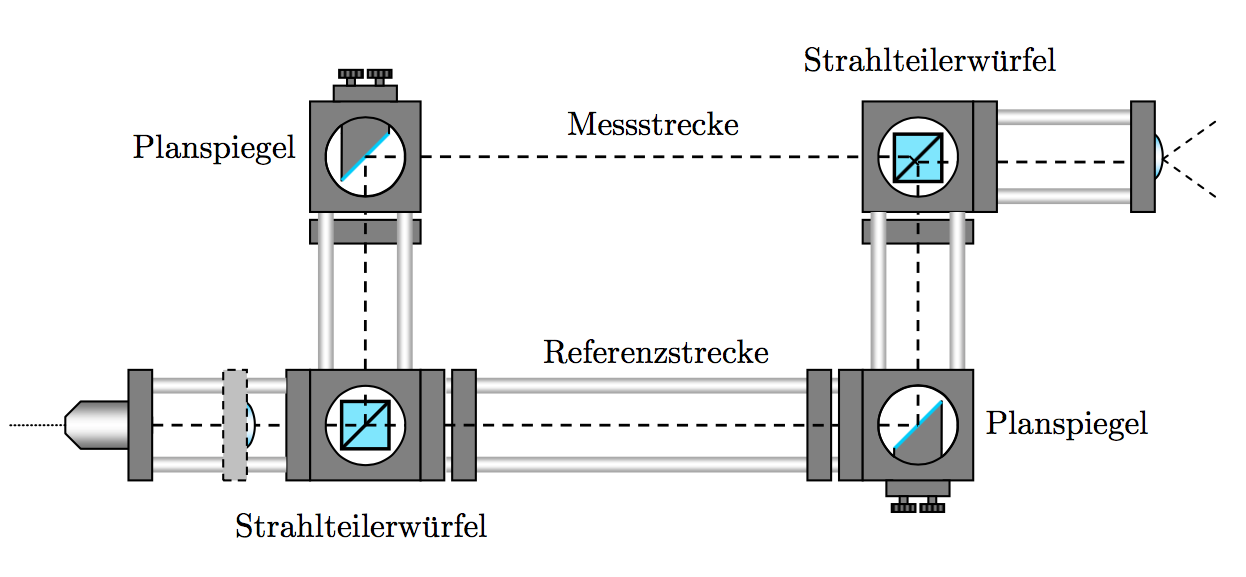
\includegraphics[width=\linewidth]{img/skizze_mzinterferometer.png}
	\caption{Prinzip - Mach-Zehnder-Interferometer}
	\label{fig:skizze}	
\end{figure}

\begin{figure}[h!]
	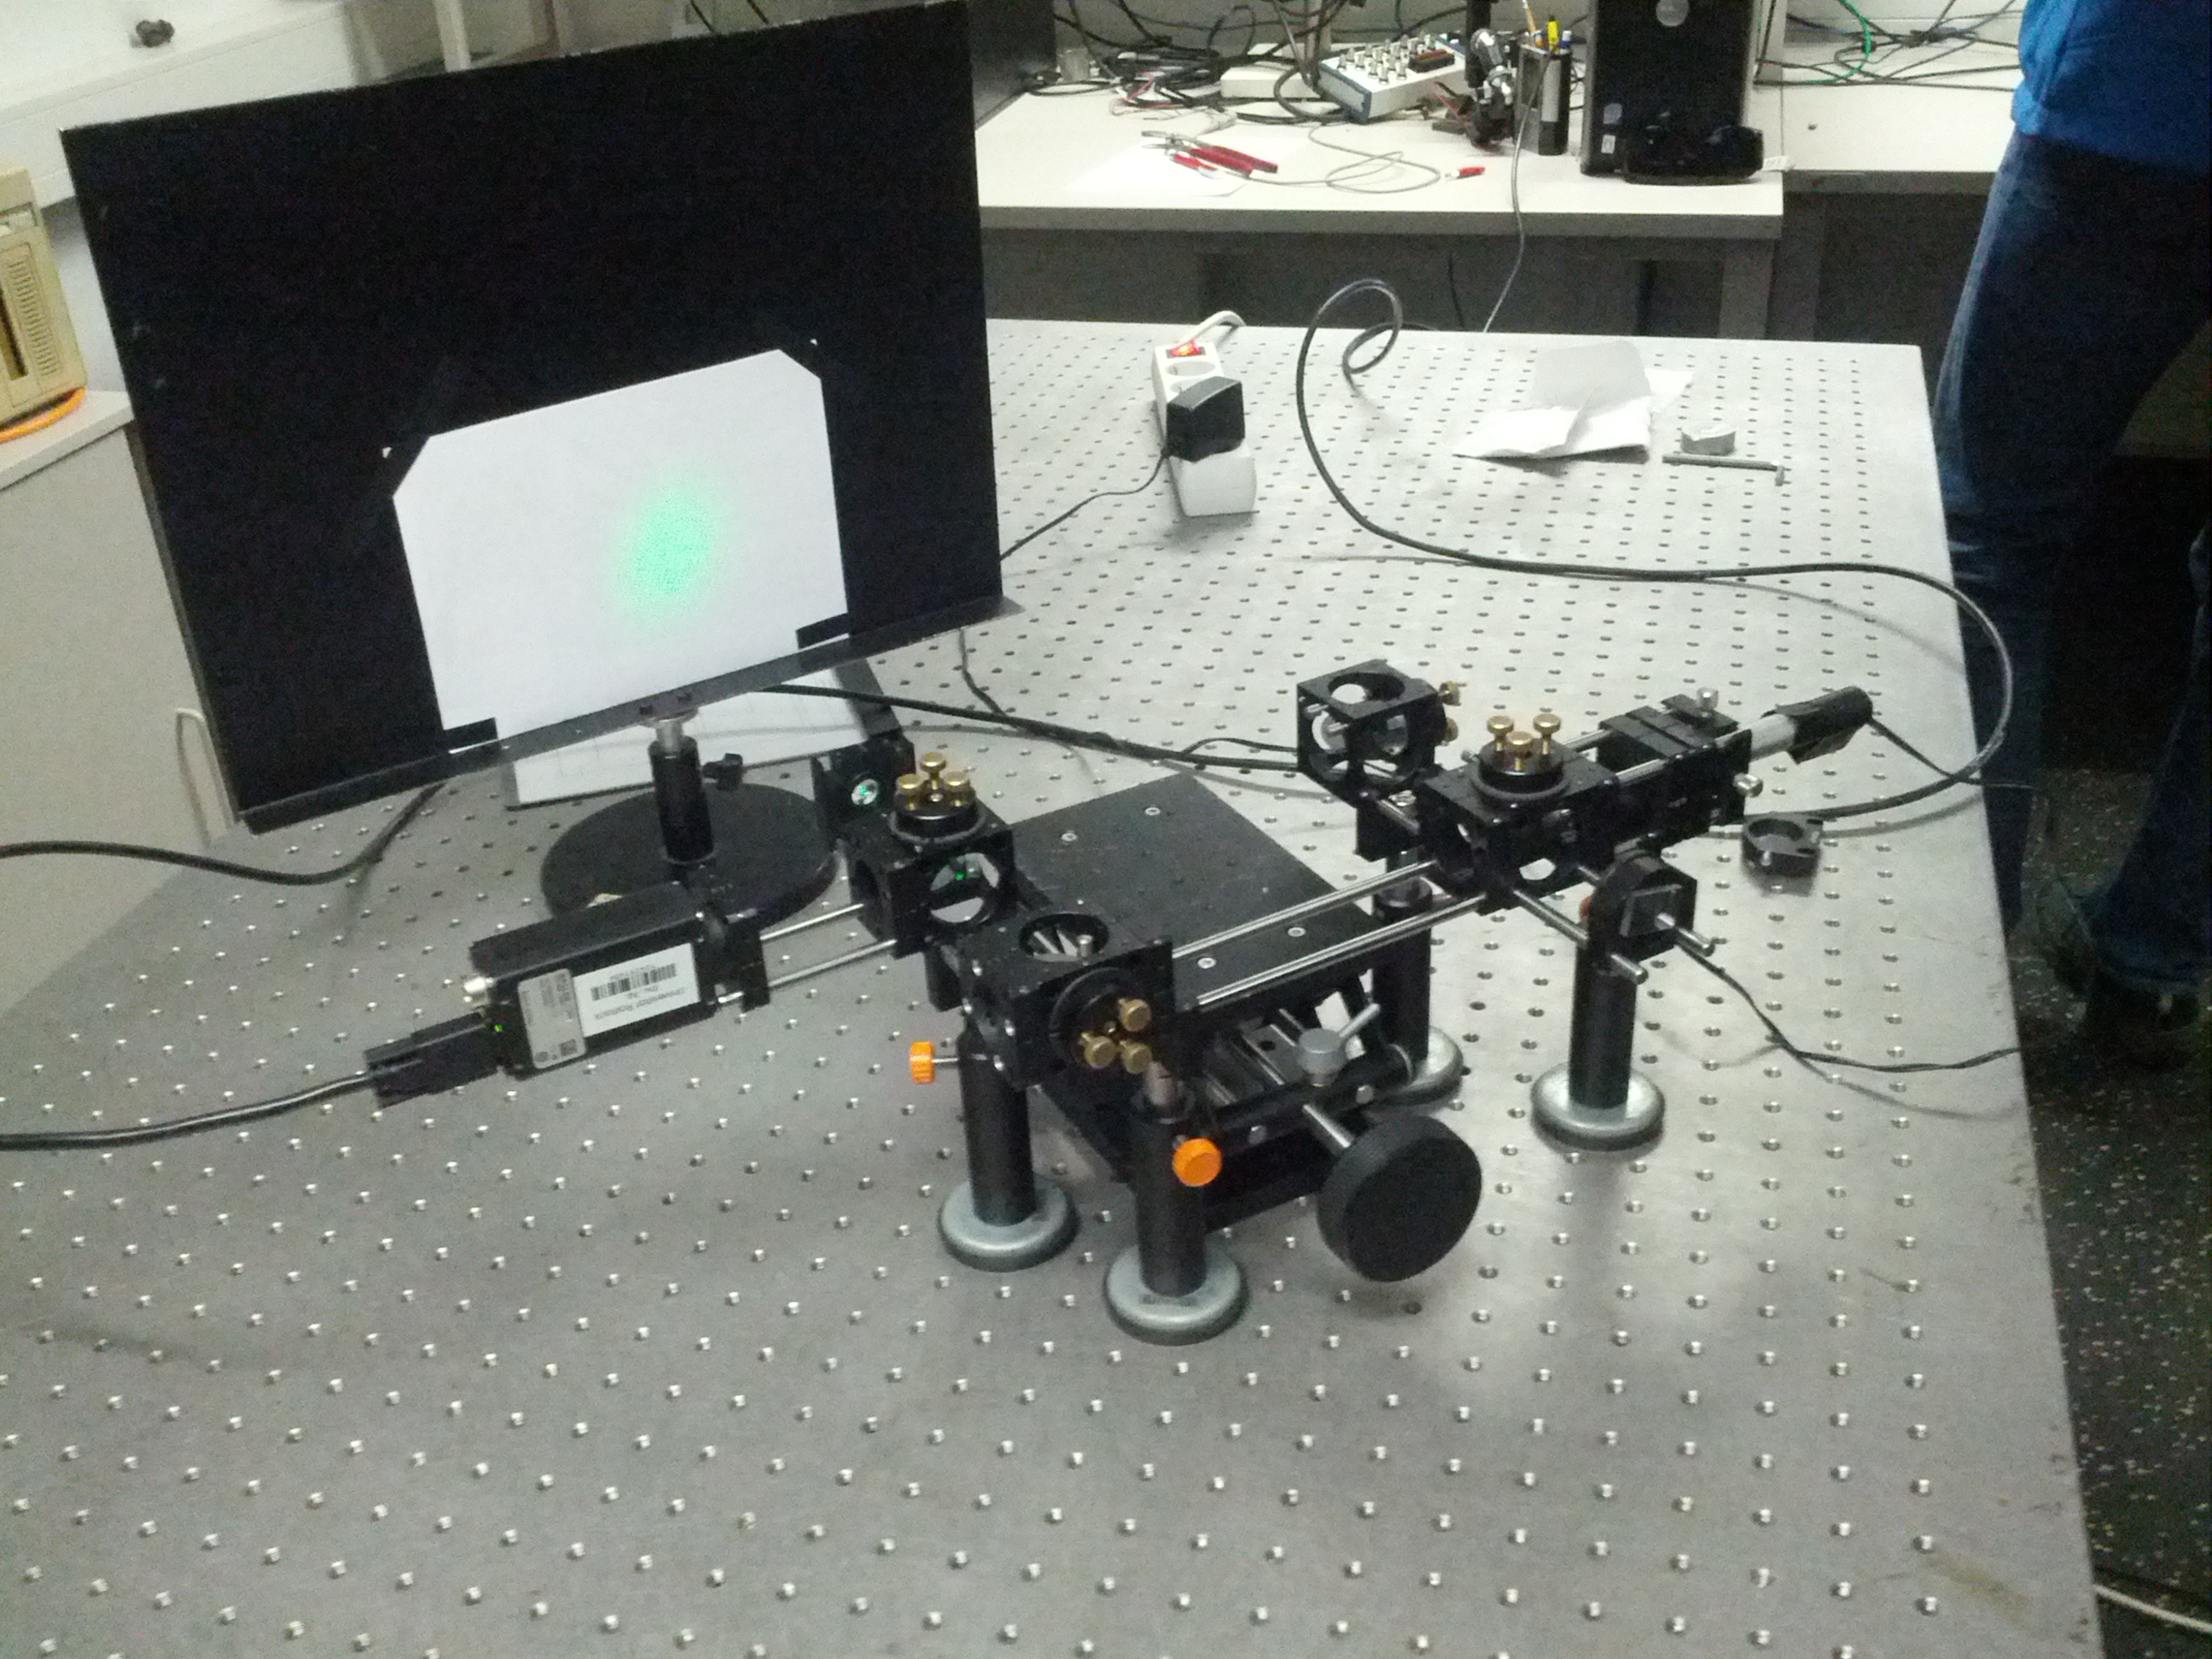
\includegraphics[width=\linewidth]{img/interferometer_aufbau}
	\caption{Versuchsaufbau - Mach-Zehnder-Interferometer}
	\label{fig:aufbau}	
\end{figure}

Um das Interferenzmuster elektronisch erfassen zu können wurde eine Kamera in einen der beiden Ausgangsstrahlen des hinteren Strahlteilerwürfels gesetzt. Zur Veranschaulichung wurde ebenfalls eine Linse im Weg des zweiten Ausgangsstrahls platziert, um das Interferenzmuster auf einem Schirm abbilden zu können (siehe Abbildung~\ref{fig:aufbau}).

Die genaue Positionierung der Strahlen erfolgte in jedem Strahlenpfad durch temporäres Einsetzten eines Pinholes und feiner Justage der optischen Komponenten. Die Strahlen wurden also alle auf dieselbe Höhe eingestellt und in der Mitte der Strecken im Mikro-Bank-System positioniert.

Für die Messung der Dickenänderung musste zunächst für jeden Durchlauf ein Referenzbild ohne ein Objekt in der Messstrecke aufgenommen werden. Anschließend wurde ein weiteres Bild aufgenommen, dass die Änderung des Interferenzmusters durch ein Objekt im Messpfad zeigte. 

Die Auswertung der Messung erfolgte in MathCad. Für die Berechnung musste eine einzelne geeignete Pixelzeile oder -spalten innerhalb der Bilder ausgewählt werden. Diese Messungen erfolgten für eine herkömmliche Brille, eine Laserschutzbrille und eine Linse.

Zur Veranschaulichung des praktischen Einsatzes eines Mach-Zehnder-Interferomters im Bereich der Temperaturmessung wurde am Ende noch eine Kerze in der Messstrecke positioniert.
	
	\clearpage
	\section{Auswertung}

Die Auswertung erfolgte in MathCad anhand der per Kamera aufgenommenen Bilder.

Zunächst wurde sich für eine qualitativ geeignete Bildzeile mit möglichst wenig Störungen entschieden. Es folgte ein Auslesen des Interferenzmusters über die Helligkeitswerte, um ein von der Bildspalte abhängiges Signal $P(s)$ zu erhalten; hierfür wurden geeignete Filter zur Elimination der Störungen verwendet. Aus dem erhaltenen (reellen) Signal wurde per Hilberttransformation das analytische Signal $P_c(s) = P(s) + \mathrm j \mathcal H\left\lbrace P(s) \right\rbrace$ generiert, das nun Phaseninformationen $\varphi(s)=\arg P_c(s)$ enthielt. Anschließend wurde aus der Phasendifferenz $\Delta\varphi(s)$  zwischen den beiden Signalen die Dickendifferenz $\Delta\varphi\lambda_0 / 2\pi n_M$ errechnet. Die jeweils letzten Diagramme der Anhänge zeigen den Verlauf der Dickendifferenz über die Breite des Laserstrahls.

In diesem Versuch wurden drei Objekte vermessen:

\paragraph*{Handelsübliche Brille (\texttt{brille2.bmp})}

\paragraph*{Laserschutzbrille (\texttt{laserbrille3.bmp})}

\paragraph*{Linse (\texttt{linse4.bmp})}
	
	\clearpage
	\section{Anhang}

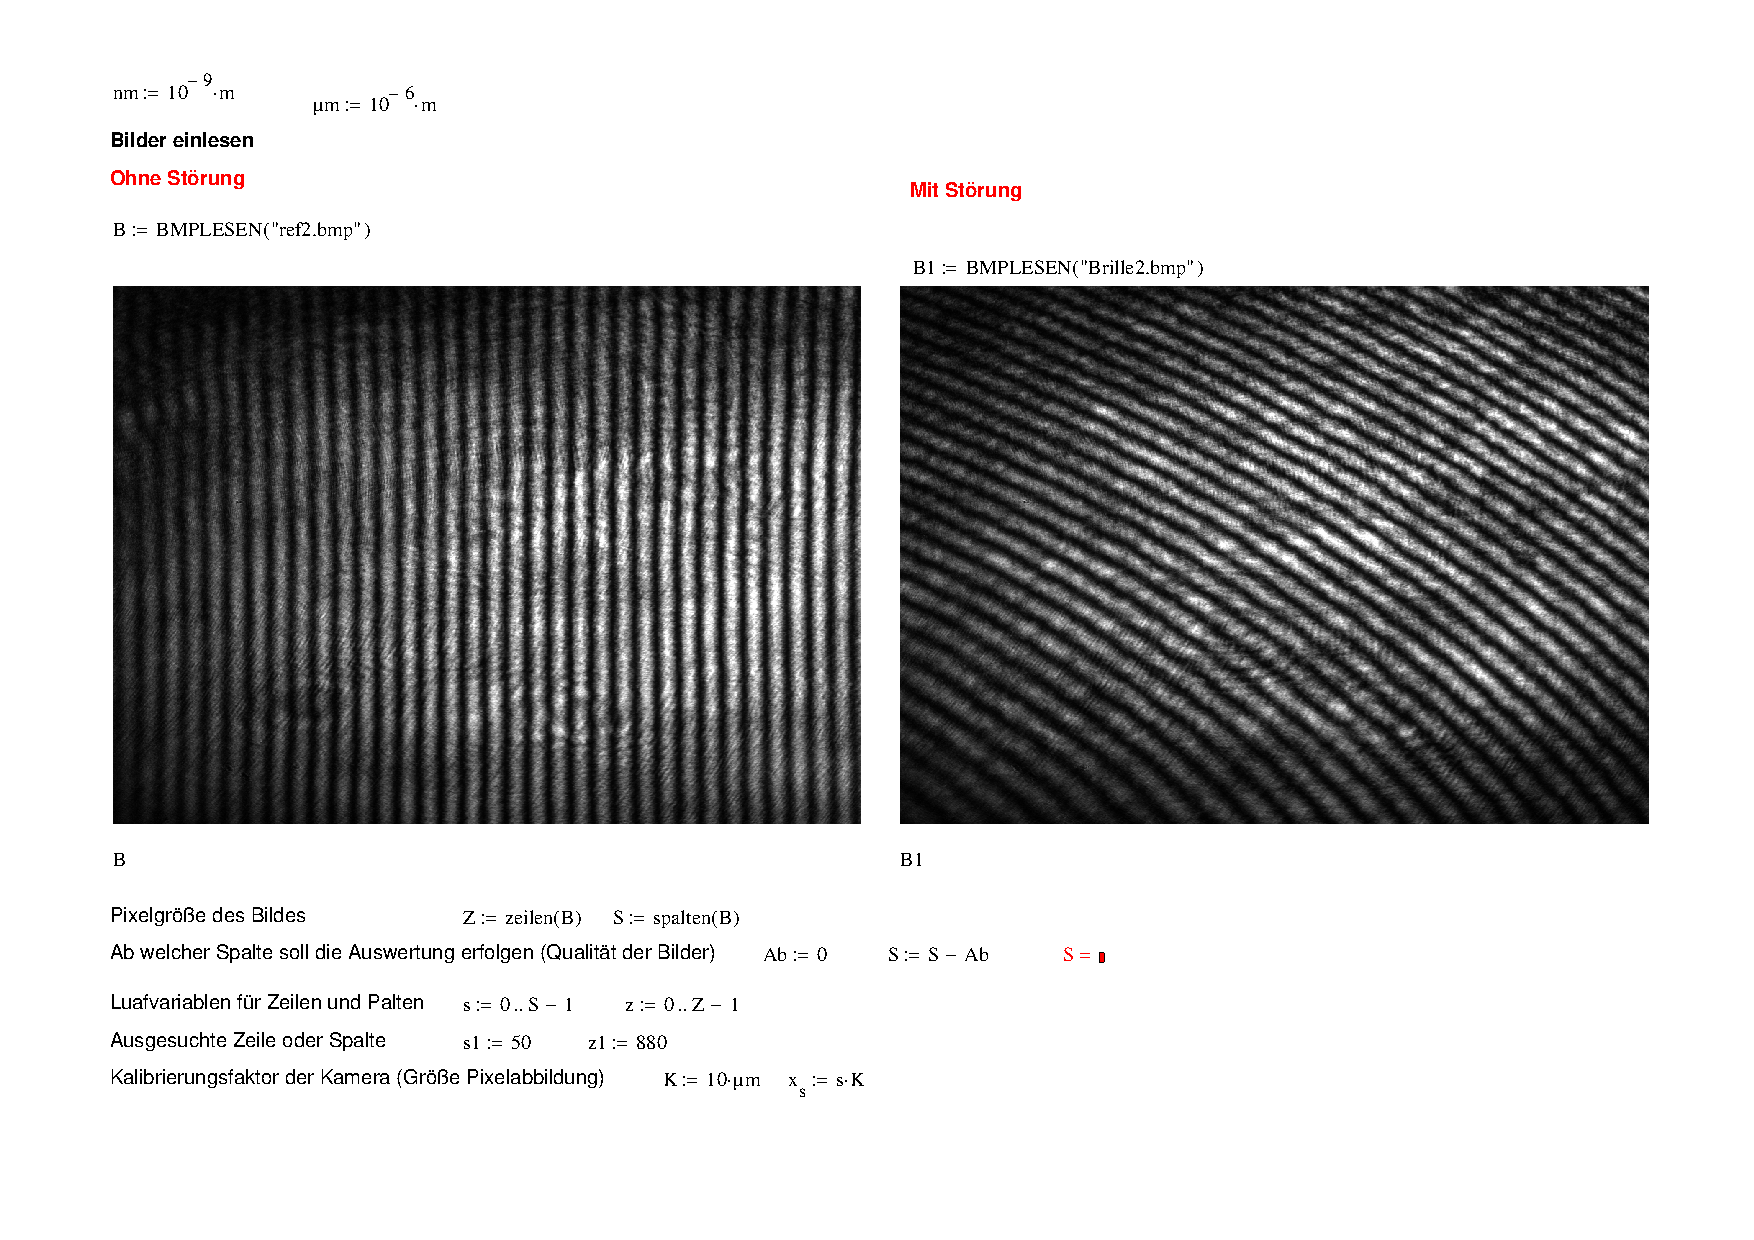
\includepdf[pages={1-6}, nup=1x2]{pdf/messreihe2.pdf}

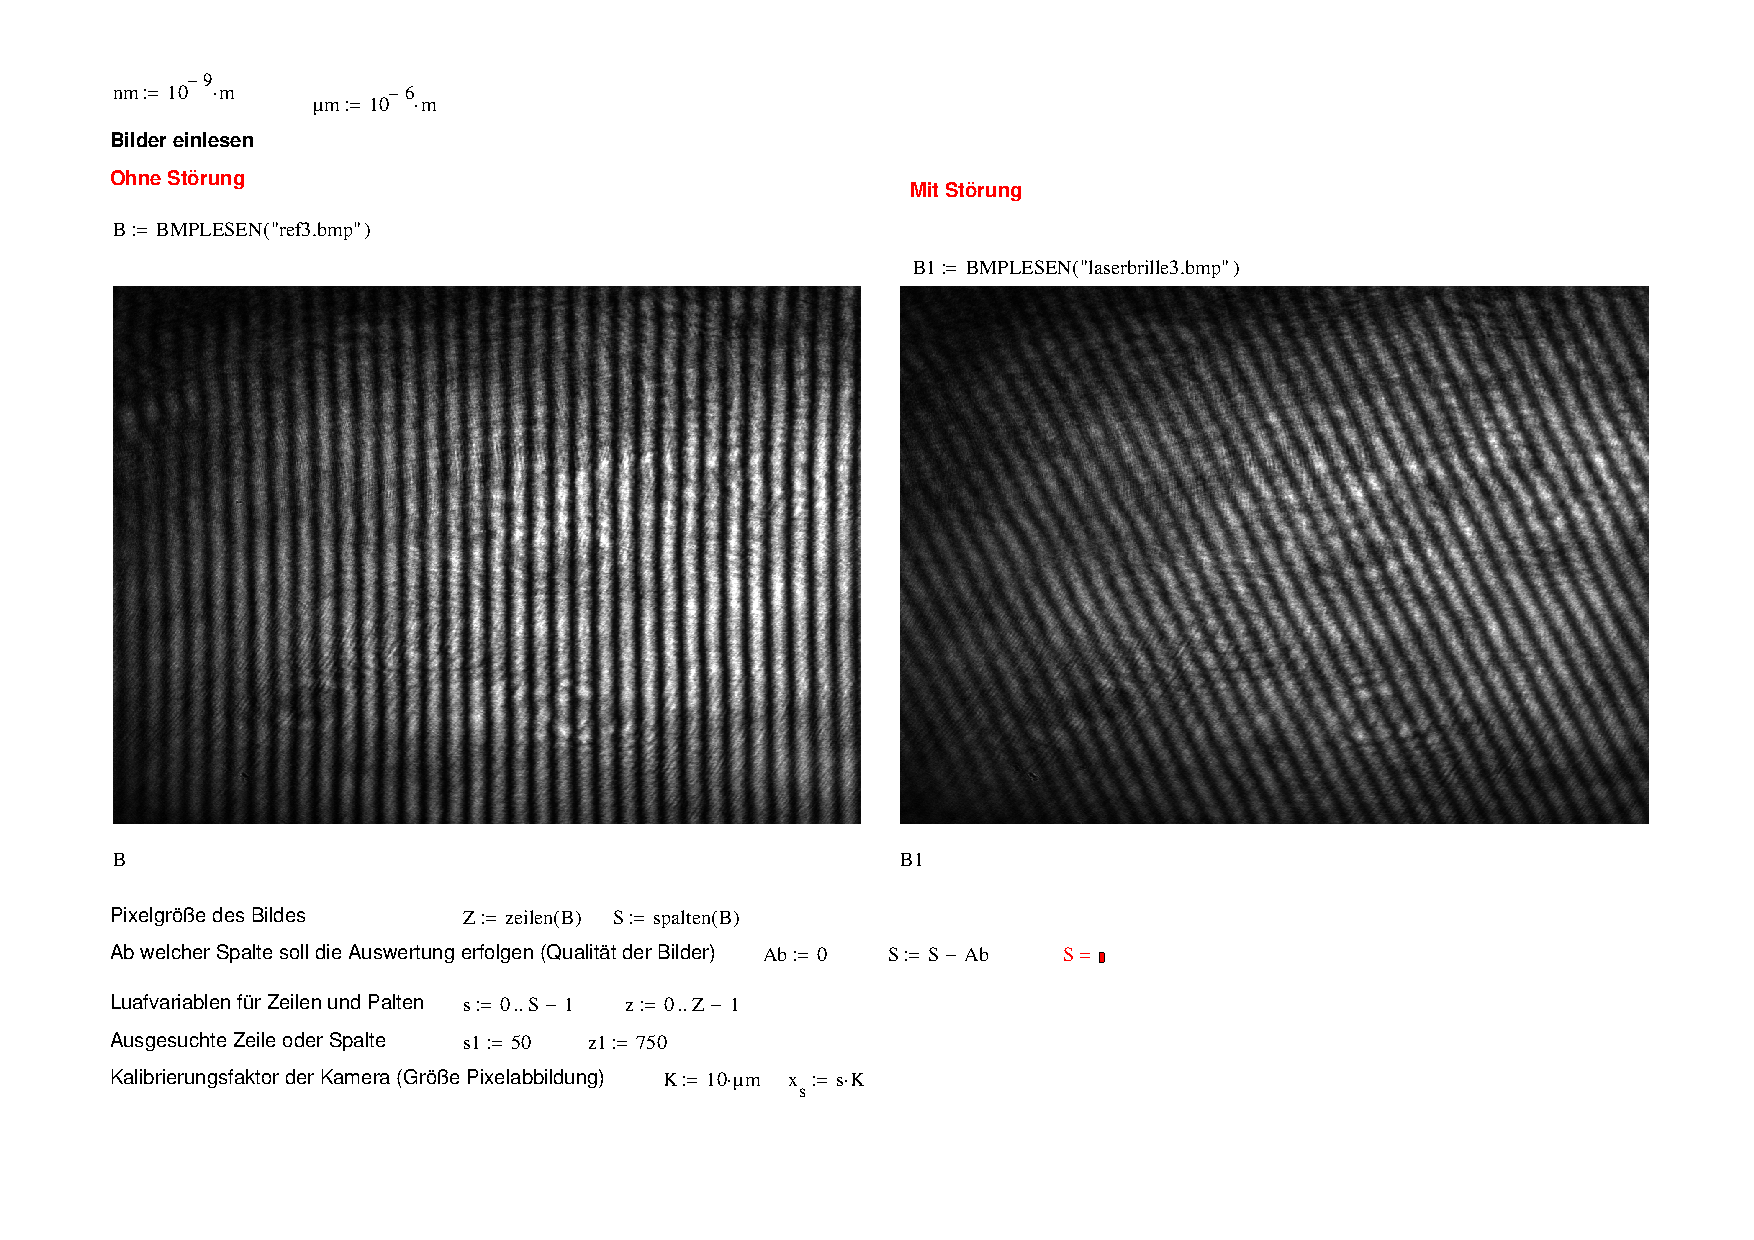
\includepdf[pages={1-6}, nup=1x2]{pdf/messreihe3_laserbrille.pdf}

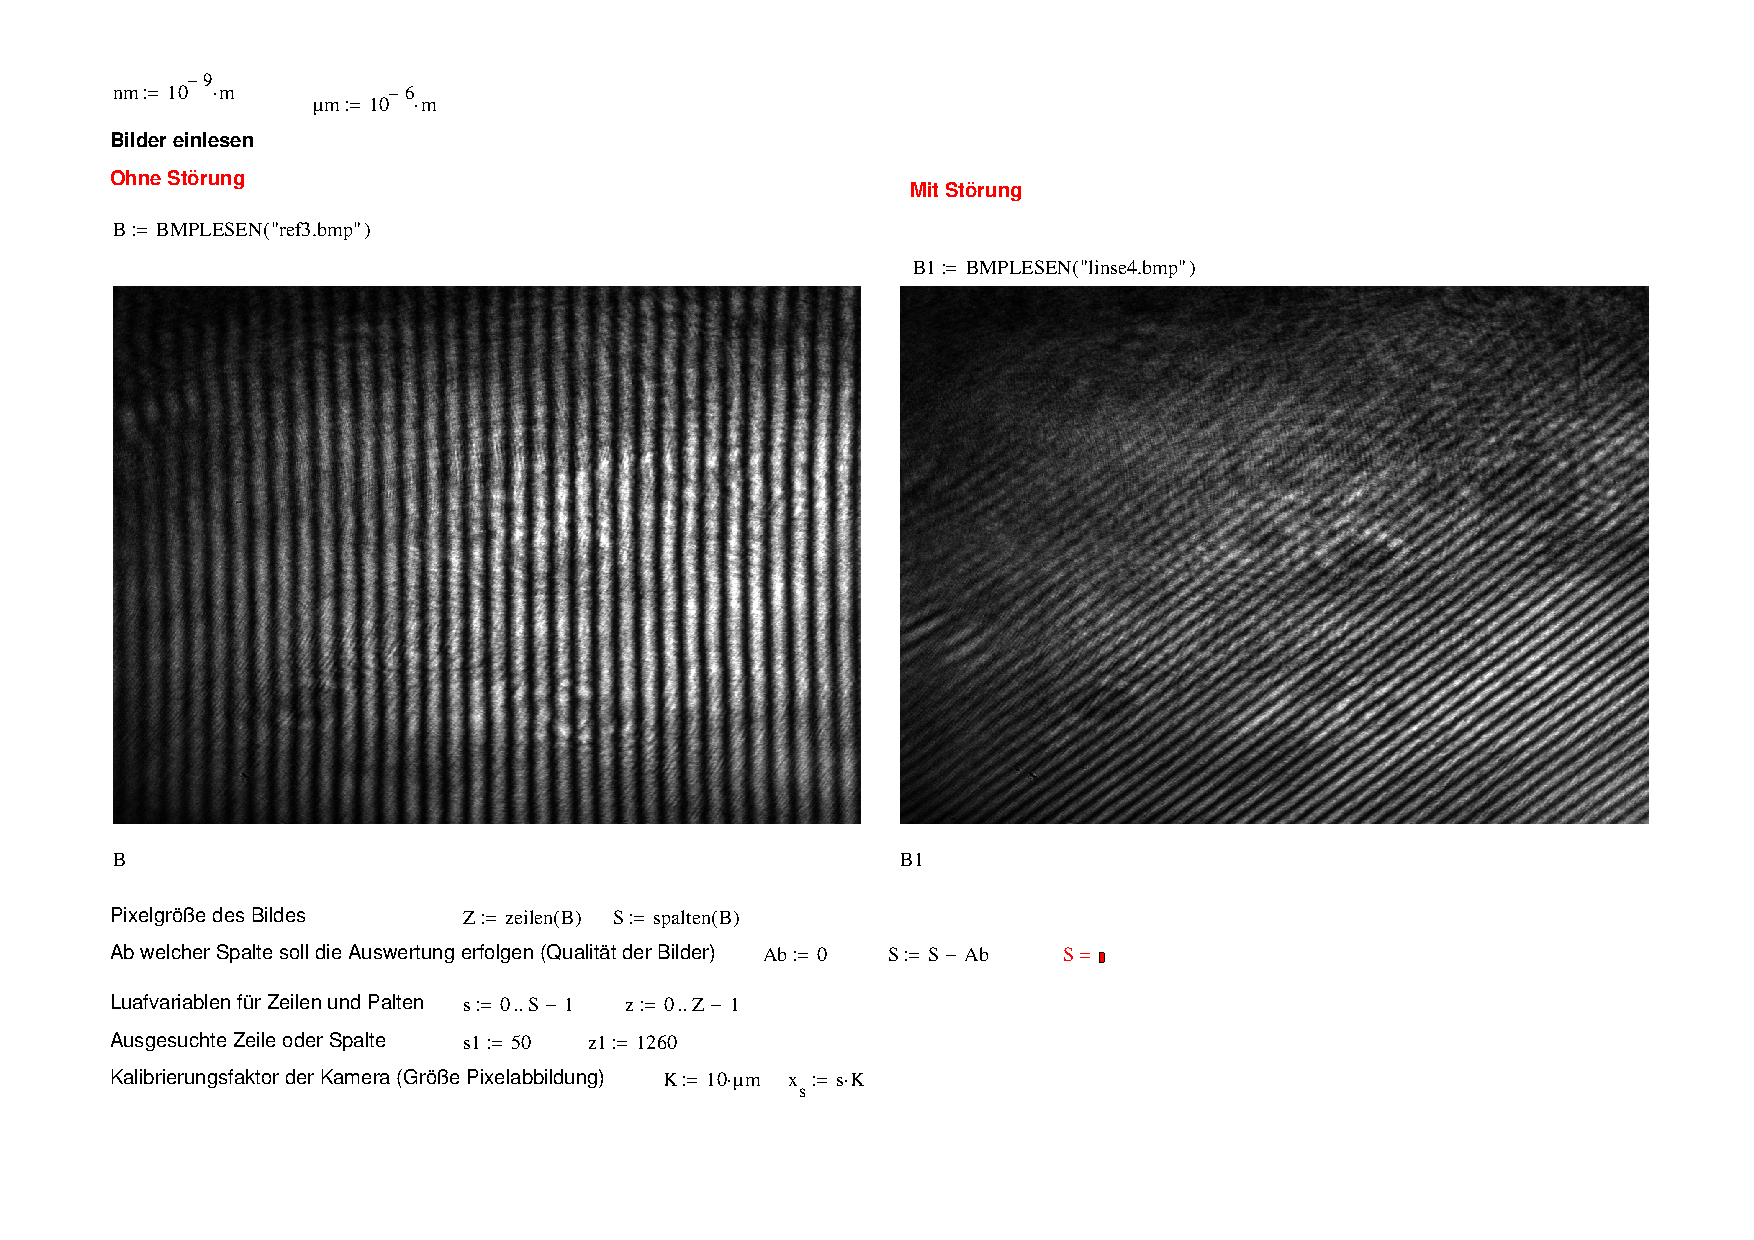
\includepdf[pages={1-6}, nup=1x2]{pdf/messreihe4_linse.pdf}
	
\end{document}
